\section{ENERGY-EFFICIENT POWER BUDGETING FOR MULTI-CORE DARK SILICON SYSTEMS}

Power budgeting, by the name, provides a power budget, which servers as a guidance and constraint for the system. The power budget in dark silicon includes the active core distribution and the corresponding DVFS stages of active cores. Typically, the given power budget should be conservative in order to keep the system in thermally safe state. The energy-efficient power budgeting gives a power budget not only keeps the system thermally safe, but also maximizes the energy efficiency of the system while keeping the power budget as high as possible.


The energy-efficient dynamic power budgeting aims to find the optimal active core distributions and their corresponding DVFS stages, which can maximize the PPW of the multi-core system. While some systems may have constraints other than thermal constraint, such as total power supply limit. But the dark silicon systems are extremely thermal limited, therefore, we focus on the major problem of thermal limits, and other constraints can be added with minor modification if needed.

PPW is defined as the ratio of the total performance (MIPS) to the total power.
\begin{equation}\label{eq:ppw}
\text{PPW} = \frac{\left \| s \right \|_{1}}{\left \| P \right \|_{1}}
\end{equation}

$s$ stands for the performance of the system in MIPS, which can be converted to the operating frequency $f$ of the active cores. Then the energy-efficient power budgeting problem can be formulated as the following optimization problem
\begin{equation}\label{eq:opt_ppw}
\begin{split}
\text{maximize } & \text{PPW} = \frac{\left \| f \right \|_{1}}{\left \| P \right \|_{1}}\\
\text{subject to} &\left\{
\begin{array}{lr}
\text{card}(P) = n_{a},\\
T_{c} \preceq T_{th}.\\
\end{array}
\right.
\end{split}
\end{equation}
where $T_{th} \in \mathbb{R}^{n}$ is the temperature rise threshold vector containing the maximum allowed temperature rises from the ambient temperature; card$(P)$ means the cardinality or size of the vector $P$, which is defined as the number of the nonzero components in $P$. In our case, card$(P) = n_{a}$ means there are $n_{a}$ active cores.

Before we solve this optimization problem, in Appendix A, for a fixed active core distribution we prove that $\text{PPW}=\frac{\left \| f \right \|_{1}}{\left \| P \right \|_{1}}$ is a quasi-concave function of the operating frequency $f$, which can make sure the optimization problem has a unique solution of $f$ that maximizes PPW.

To find the unique solution for the optimization problem in \eqref{eq:opt_ppw} is very hard, because of the high computational complexity of the problem, which comes from the fact that the cores have thermal impact on each other, changing the DVFS stage of one core not only would change the PPW of the core itself, but would also change the temperature rise of other cores, therefore changing the PPW of them, which makes enumerating all possible active core distribution and DVFS stages the only way to obtain the optimal solution. Therefore, we need to transform this problem into a problem with low complexity.

We can prove $T$ is convex w.r.t $f$, considering for a fixed active core distribution, there is a unique $f$ that can maximize PPW. Therefore, for a fixed active core distribution, a unique temperature vector, denoted by $T_{opt}$, that can maximize PPW also exists. However, $T_{opt}$ only works for a fixed active core distribution, obtaining $T_{opt}$ for each active core distribution only complicates the problem. Therefore, we want to obtain one or several $\hat{T}_{opt}$, different from $T_{opt}$, which only works for a fixed active core distribution, and includes the optimal temperature distribution for all cores on and off, $\hat{T}_{opt}$ works for all active core distributions or a defined range of scenarios, and the elements in $\hat{T}_{opt}$ are the optimal temperatures that lead to optimal PPW for each core.


The closer $T_{c}$ is to $\hat{T}_{opt}$, the higher the PPW. So instead of
directly maximizing PPW, the optimization problem in \eqref{eq:opt_ppw} can be transformed to minimizing the difference between $T_{c}$ and $\hat{T}_{opt}$:
\begin{equation}\label{eq:ppw_minimize_t}
\begin{split}
\text{minimize } &  \left \| \hat{T}_{opt}-T_{c} \right \|_{2}\\
\text{subject to} &\left\{
\begin{array}{lr}
\text{card}(P) = n_{a},\\
T_{c} \preceq T_{th}.\\
\end{array}
\right.
\end{split}
\end{equation}


Considering the thermal interaction between cores, it's not straightforward to obtain the $\hat{T}_{opt}$ for all cores. A method to calculate $\hat{T}_{opt}$ efficiently is shown in next section.

\subsection{Obtaining optimal temperature for each core}
Due to the thermal impact active cores have on each other, changing the temperature of core $i$ will change the temperature of other cores, which will in turn change the temperature of core $i$. If we can isolate each of the core, the optimal temperature can be calculated easily. However, the optimal temperature we obtained for isolated cores deviate from the real optimal temperature, and can cause large error in dark silicon system. Therefore, an efficient method to calculate $\hat{T}_{opt}$ for isolated cores and a temperature compensation method to correct the error are proposed in this section.

\subsubsection{Calculating optimal temperature for isolated cores}
In order to isolate the cores, we first express the PPW of a single core $i$ in steady state as:
\begin{equation}\label{eq:min_ppw}
\text{PPW}=\frac{f}{p_{d}+p_{s}},
\end{equation}

By integrating the linearized subthreshold current $I_{sub}$ in \eqref{eq:lin_leakage} into \eqref{eq:min_ppw}, we have

\begin{equation}\label{eq:1_ppw}
\text{PPW} = \frac{f}{p_{d}+V_{dd}(a_{s}(T_{i}+T_{a})+p_{0})}.
\end{equation}

Note that, the temperature rise $T_{i}$ of the single core in \eqref{eq:1_ppw} is composed of the temperature rise caused by the core itself $T_{self}$, the temperature rise caused by other active cores $T_{other}$, $T_{a}$ is the ambient temperature. In order to isolate core $i$, we have to express the temperature rise of core $i$ with only the power of core $i$ itself.

Let's begin with calculating the temperature rise $T_{c}$ of the chip, considering the calculation is done in steady state, the differential term $C\frac{dT(t)}{dt}$ is neglected in \eqref{eq:gt}, leading to
\begin{equation}\label{eq:tc}
T_{c} = B^{T}G^{-1}BP.
\end{equation}
Let $A = B^{T}G^{-1}B \in \mathbb{R}^{n \times n}$ to simplify notation, please note that, compared to $G$ matrix, although the size of $A$ matrix is reduced, all thermal model information including packages are reserved. The simplified 
\eqref{eq:tc} can be expressed as
\begin{equation}\label{sim_tc}
\begin{split}
T_{c} &= AP,\\
&=
{\left[
\begin{matrix}
 a_{11} & a_{12} & \cdots & a_{1n} \\
 a_{21} & a_{22} & \cdots & a_{2n} \\
 \vdots & \vdots & \ddots & \vdots \\
 a_{n1} & a_{n2} & \cdots & a_{nn} \\
\end{matrix}
\right]}
{\left[
\begin{matrix}
 p_{1}   \\
 p_{2}   \\
 \vdots  \\
 p_{n}   \\
\end{matrix}
\right]}.\\
\end{split}
\end{equation}

As \eqref{sim_tc} shows, the temperature rise $T_{i}$ can be expressed as
\begin{equation}\label{eq:ti}
T_{i} =a_{i1}p_{1} + a_{i2}p_{2} +\cdots + a_{in}p_{n}. 
\end{equation}

Therefore, the diagonal elements $a_{ii}$ in $A$ can be seen as the thermal resistance of core $i$ itself, and the non-diagonal elements $a_{ij}$ in $A$ can be seen as the thermal resistance between core $i$ and $j$. The diagonal element $a_{ii}$ can be extracted from $A$ to calculate the temperature rise of isolated core $i$ as:
\begin{equation}\label{eq:t_ap}
\begin{split}
T_{i}&\approx a_{ii} \cdot p_{i}\\
&=a_{ii}(p_{d}+p_{s})
\end{split}
\end{equation}

By substituting $T_{i}$ in \eqref{eq:1_ppw} with \eqref{eq:t_ap}, we can have:
\begin{equation}\label{eq:1_ppw_2}
\text{PPW} = \frac{f(1-a_{ii} \cdot a_{s} \cdot V_{dd})}{V_{dd}(a_{s}\cdot T_{a}+p_{0})+p_{d}},
\end{equation}
which eliminates the thermal impact of other active cores. As proved in Appendix, PPW is a quasi-concave function of operating frequency $f$, the optimal operating frequency $f$ that leads to maximum PPW for core $i$ can be obtained with standard gradient search techniques~\cite{Boyd:Convex_BOOK'06} from \eqref{eq:1_ppw_2}. Because $T$ is convex w.r.t $f$, the optimal temperature can be calculated with optimal $f$.

\begin{figure}
\centering

\includegraphics[width=0.46\linewidth]{fig/unique_position.eps}
\caption{$3$ kinds of cores based on their positions in the system for a $16$-core system.}
\label{fig:unique_position}
\end{figure}

Note that we do not need to repeat the calculating process for all cores to obtain all the optimal temperature. All cores can be divided into several kinds based on their position in the system, for a $16$-core system, there are only $3$ kinds of cores which are shown in Fig.\ref{fig:unique_position}. The cores of the same kind share the same diagonal elements in $A$ matrix. Therefore, calculating the optimal temperature for each kind of core instead of all cores can greatly reduce the computation time.

However, the optimal temperature obtained for isolated cores ignores the thermal impact of other active cores, which is only accurate when there is only $1$ active core. For cases with active cores more than $1$, the temperature rise caused by other active cores will make the optimal temperature deviate from the one we obtained from \eqref{eq:1_ppw_2}. Also, for different active core distributions, the thermal impact active cores have on each other will be different, the $T_{opt}$ is different. Therefore, a compensation method is need to correct the error induced by different active core number and active core distribution.


% Maximum PPW can be obtained if the calculated energy-efficient power budget is applied to each of the active cores, no matter what active core distribution it is. 

% \begin{figure}
%   \centering
%   \subfigure[MIPS = 246.3, MIPS/Watt = 2.6]{
%     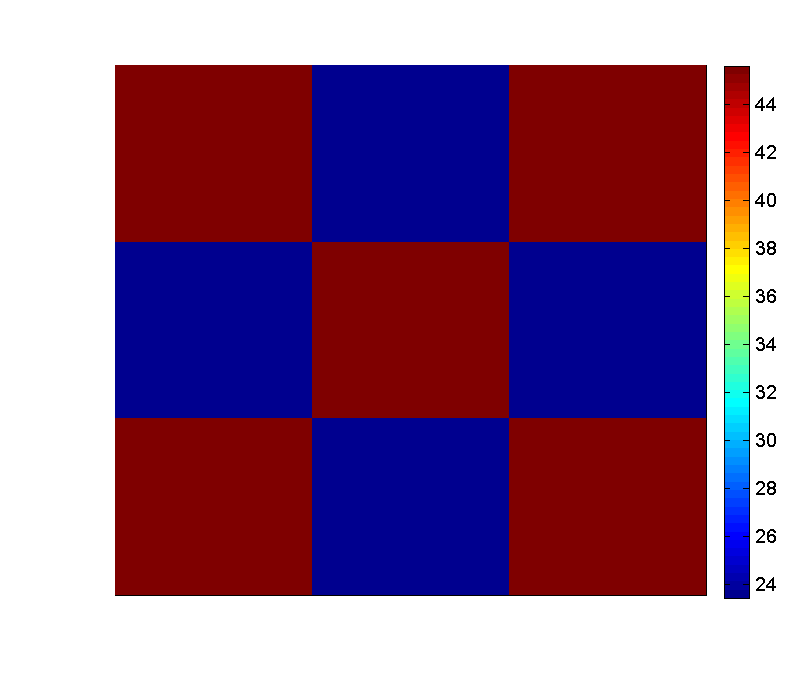
\includegraphics[width=0.46\columnwidth]{fig/opt_tem_1.eps}\label{fig:opt_tem_1}
%   }
%   \hspace{1ex}
%   \subfigure[MIPS = 215.6, MIPS/Watt = 2.6]{
%     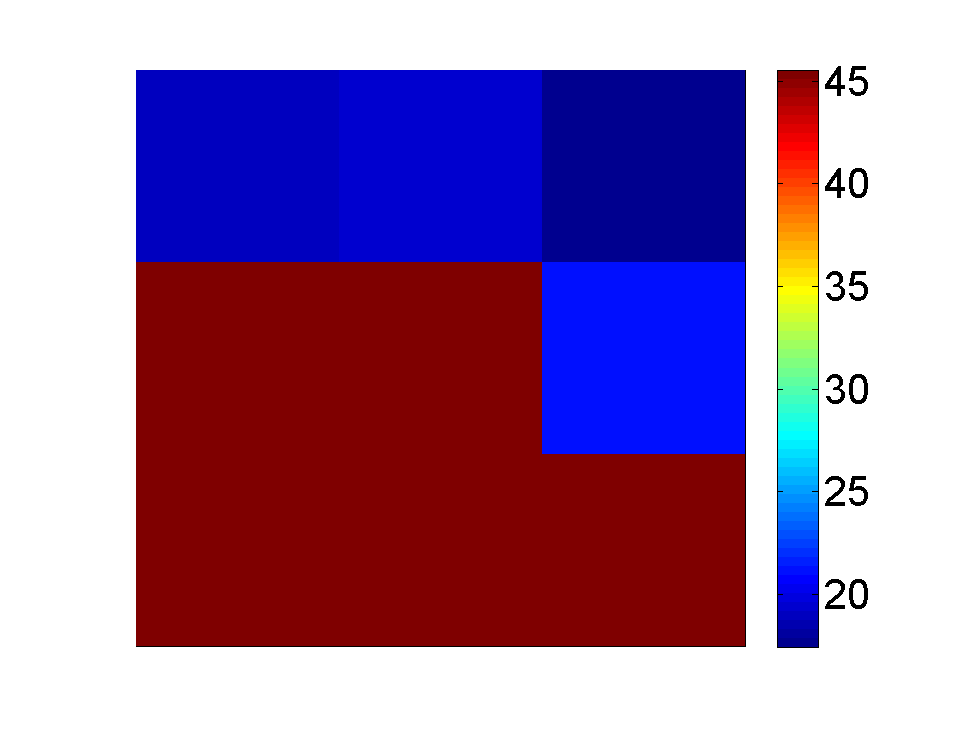
\includegraphics[width=0.46\columnwidth]{fig/opt_tem_2.eps}\label{fig:opt_tem_2}
%   }
%   \caption{Temperature distributions of a 9-core system with 5 cores active in maximum energy efficiency.}
%   \label{fig:opt_tem}
% \end{figure}

% For the last observation, we also provide experimental evidence in addition. We use Monte Carlo method, by fixing active core number and distribution, only changing the DVFS stages of active cores, we obtain the optimal DVFS stages of each active cores that leads to maximum energy efficiency for several fixed active core distributions. The Monte Carlo simulation number for each fixed active core distribution is $10000$. The corresponding temperature distribution is plotted in Fig.~\ref{fig:opt_tem}, in which the temperature distributions of a $9$-core system with $5$ active cores are shown. 

% As can be seen, the optimal energy efficiency of both Fig.~\ref{fig:opt_tem_1} and Fig.~\ref{fig:opt_tem_2} are relatively the same, although the active core distribution is not the same for them, which means that the active core distribution that corresponds to optimal energy efficiency is not unique. However, for different active core distributions, the throughput while in optimal energy efficiency are not the same.





\subsubsection{Calculating optimal temperature for isolated cores with temperature compensation}
The optimal temperature calculated in previous section does not consider of other cores' thermal impact, which could cause major error in dark silicon system, where the temperature rise caused by other cores could make up of a considerable part of the whole temperature rise. Therefore, a compensation method to modify the isolated core's temperature rise $T_{i}$ is proposed in this section.

% \begin{equation}\label{eq:c_full_1_ppw}
% \text{PPW}=\frac{f}{p_{d}+V_{dd}(a_{s}((1+\lambda)T_{i}+T_{a})+p_{0})}.
% \end{equation}
\begin{equation}\label{eq:t_compensation}
\begin{split}
T_{i} &=a_{i1}p_{1} + a_{i2}p_{2} +\cdots + a_{in}p_{n},\\
&\approx(1+\lambda)a_{ii}p_{i}.
\end{split}
\end{equation}

The basic idea of this method is to compensate for the temperature rise caused by other active cores in \eqref{eq:1_ppw} with a parameter $\lambda$, which stands for the temperature rise ratio induced by other active cores, as shown in \eqref{eq:t_compensation}. With $\lambda$, the thermal impact other active cores have on the isolated core can be introduced, therefore the error induced by isolation can be corrected.

The temperature compensation can be perfectly accurate, if for fixed active core distribution, for core $i$ we obtain a $\lambda$, which is calculated as:
\begin{equation}\label{eq:lambda_accuracy}
\lambda =\frac{\sum_{l=1}^{n}a_{il}p_{l}-a_{ii}p_{i}}{a_{ii}p_{i}},
\end{equation}
then the temperature rise caused by other active cores can be compensated without error, however, the overhead would be too high. We find out if we generate a $\lambda$ for each active core number for each kind of core, and assume the power of every active core are the same, the accuracy and overhead can both be satisfactory. $\lambda_{ij}$, which stand for the $\lambda$ for core $i$ when active core number is $j$ can be calculated as:
\begin{equation}\label{eq:lambda}
\lambda =\frac{j \cdot \sum_{l=1}^{n}a_{il}-a_{ii}}{a_{ii}},
\end{equation}

% The approximation accuracy of this method depends on how many $\lambda$ we generate. If for each active core distribution we generate a $\lambda_{i}$ to stand for the temperature rise ratio caused by other active cores of core $i$, then calculation would be perfectly accurate. However, the computational complexity will be too high. If we generate a single $\lambda$ to stand for the temperature rise ratio for all cores in all cases, the error would be too large, because the temperature rise induced by other active cores may vary dramatically for different active core numbers in dark silicon. 

% \begin{figure}
% \centering
% 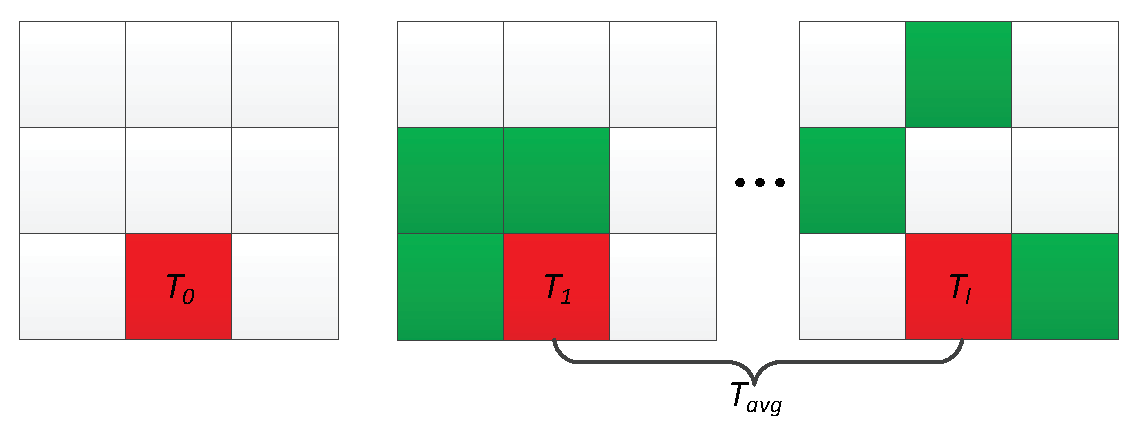
\includegraphics[width=0.9\linewidth]{fig/tavg.eps}
% \caption{The process of obtaining $\lambda$ for each active core number.}
% \label{fig:tavg}
% \end{figure}

\begin{table}
  \caption{The energy-efficient power budget induced temperature error for cases with and without $\lambda$. The fixed core is the $1^{st}$ core, for each active core number, $50$ random active core distributions are generated.}
  \label{tab:compensation}
  \centering
  \begin{tabular}{c|c||p{1cm}<{\centering}|p{1cm}<{\centering}||p{1cm}<{\centering}|p{1cm}<{\centering}}
    \hline
    Core & Active     & \multicolumn{2}{c||}{With $\lambda$ ($^{\circ}$C)}  & \multicolumn{2}{c}{Without $\lambda$ ($^{\circ}$C)}\\
\cline{3-6}
    \#       &   \#       &  Avg    & Max &  Avg  &  Max  \\
     \hline
\hline
  \multirow{3}{*}{9} &      2       &   1.1  &   1.9 &2.1&4.0\\
             &      4       &    1.3    &   2.7  &7.0&11.7 \\
             &      7       &   1.2     &   2.2   &13.7&16.1\\
     \hline
   \multirow{3}{*}{16} &      3        &   0.3 &   0.7   &1.5 &2.2 \\   
             &      8       &    0.5     &  1.2  &7.2 &8.3   \\
             &      13     &     0.4    &   1.2  &12.9 &13.7 \\
     \hline
  \multirow{3}{*}{25} &      5       &    0.4 & 1.1 & 3.2 &  4.2   \\ 
              &     12      &    0.5     &    1.4   &  8.7 & 9.9 \\
              &     20      &    0.4     &    1.1   & 13.5 & 14.1 \\ 
     \hline
  \multirow{3}{*}{36}  &     8        &    0.4  &    1.1 & 4.1 & 5.6\\
              &     18      &   0.5      &   1.6  & 10.0 & 11.4  \\
              &     28      &    0.4     &   0.9 & 14.4 & 15.2\\
     \hline
  \multirow{3}{*}{64}  &     12      &   0.4  &   1.2  & 3.8 &4.9 \\
              &     32      &    0.5     &     1.6   & 9.6 & 10.6   \\
              &     52      &     0.4   &     1.0   & 15.9 & 16.5\\
 \hline 
\multirow{3}{*}{100}  & 16 & 	 0.5&	1.1& 3.3 &  4.3\\
                      & 52 &	 0.7&	1.7& 11.4 & 13.0\\
                      & 76 &	 0.5&	1.8& 16.6 & 17.6\\
\hline
\end{tabular}
\end{table}


% As shown in Fig.~\ref{fig:tavg}, for core $i$, to obtain its $\lambda$ for $4$ active cores, first we calculate the temperature rise $T_{0}$ with core $i$ being the only active core. Then we generate several random active cores distributions with $4$ active cores, and core $i$ is always included in active cores. Note that the power of all active cores are set to be the same. By comparing the averaged temperature rise $T_{avg}$ of core $i$ in the random distributions with $T_{0}$, $\lambda$ for core $i$ with $4$ active cores can be obtained:
% \begin{equation}\label{eq:lambda}
% \lambda = \frac{T_{avg}-T_{0}}{T_{0}}.
% \end{equation}

By repeating the process, we can generate a matrix $\Lambda$, in which $\lambda_{ij}$ stands for the compensation parameter for core $i$ when the active core number is $j$. We substitute the $T_{i}$ in \eqref{eq:1_ppw} with the compensated temperature in \eqref{eq:t_compensation} and get:
\begin{equation}\label{eq:1_ppw_3}
\begin{split}
\text{PPW} =& (\frac{(1+\lambda)(V_{dd}(a_{s}\cdot T_{a}+p_{0})+p_{d})}{f(1-a_{ii} \cdot a_{s} \cdot V_{dd})}\\
&-\frac{\lambda(p_{d}+V_{dd}(a_{s}\cdot T_{a}+p_{0}))}{f})^{-1},
\end{split}
\end{equation}

By solving \eqref{eq:c_full_1_ppw} for every $\lambda$, the energy-efficient optimal temperature matrix can be obtained, in which $T_{ij}$ stands for the optimal temperature for core $i$ when the active core number is $j$.

In order to test the effectiveness of $\lambda$, for example, we first choose a $9$-core system with $4$ active cores, several active core distributions can be generated with core $i$ always turned on. We can obtain the $\lambda_{i}$ for core $i$ for each active core distribution, which is accurate, therefore the energy-efficient power budget calculated in this case can be considered "golden". We also obtain the energy-efficient power budgets calculated with $\lambda_{i4}$ and without $\lambda$ both. By comparing the power budget induced temperature of the latter $2$ cases with "golden", the effective of $\lambda$ can be verified.

In addition to the case shown above, we tested many other systems with different number of cores and active cores. The results are collected in Table~\ref{tab:compensation}.

\subsection{Energy-efficient power budgeting with optimal performance in steady state}
Now that the energy-efficient power budget for all cores in each active core number is obtained, as long as the active cores' power is as close to the corresponding $P_{opt}$ as possible, the energy efficiency of the system is maximized, no matter what active core distribution it may be. However, it's not only energy efficiency we are seeking, the throughput of the system is also an important metric, which are affected by the active core distribution greatly in dark silicon system. Therefore, the next goal of our energy-efficient power budgeting is to maximize the throughput while the energy efficiency is maximized.

Considering it's a combinational problem to find the optimal active core distribution that leads to maximum throughput, 

In \eqref{eq:opt_topt}, we have shown that we can allocate energy-efficient power budget by making the temperature of each core as close to the optimal temperature $T_{opt}$ of itself. However, \eqref{eq:opt_topt} is still a combinational problem, which is very hard to solve. In this section, a steady state example is given to show how to efficiently find a sub-optimal solution using a greedy based method. Please note that, we present our method in steady state mainly for the purpose of clarity.

We plug \eqref{sim_tc} into the optimization problem \eqref{eq:opt_topt} and get
\begin{equation}\label{eq:sim_opt_topt}
\begin{split}
\text{minimize } &  \left \| T_{opt} - AP \right \|_{2}\\
\text{subject to} &\left\{
\begin{array}{lr}
\text{card}(P) = n_{a},\\
AP \preceq T_{th}.\\
\end{array}
\right.
\end{split}
\end{equation}

Finding the optimal solution of such optimization problem requires brute force search of all possible combinations of non-zero positions in $P$ which satisfies $\text{card}(P)=n_{a}$. The high complexity of this method makes it not suitable for multi-core system with large number of cores. It is also noticed that for such systems, finding the optimal solution is not necessary. This is due to the fact that when core number is large, each core takes relatively small area, so there exist many sub-optimal active core distributions which only have slightly larger objective value (measured by cost function) than that of the optimal solution. For example, consider a $25$-core system with $13$ cores active. The optimal solution of such system is shown in xx, and one sub-optimal solution is shown in xx. This is also verified in our experiments by comparing the optimal power budget and the sub-optimal power budget, as shown later.

For a $n$-core system with $n_{a}$ active cores, the basic idea of finding such sub-optimal solution is described as follows: we first find the optimal solution for only one active core. Next, we $fix$ the first active core position determined by the first step, and find the optimal solution of two cores, with the second active core position determined. Please note that although we say "optimal" in the second step, such solution is only the optimal solution with the first active core fixed at the position determined by the first step, not the true optimal solution for general two active cores. Similarly, in the $(i+1)$-th step, we look for the optimal solution for $i+1$ active cores with the position of $i$ active cores found in all previous steps remain fixed. By proceeding such strategy for $n_{a}$ steps, we can arrive at a sub-optimal solution for $n_{a}$ active cores.


To demonstrate the greedy based method in details, we begin with finding solution for one active core. The optimization problem for one active core is
\begin{equation}\label{eq:1_sim_opt_topt}
\begin{split}
\text{minimize } &  \left \| T_{opt_1} - AP \right \|_{2}\\
\text{subject to} &\left\{
\begin{array}{lr}
\text{card}(P) = 1,\\
AP \preceq T_{th}.\\
\end{array}
\right.
\end{split}
\end{equation}


We have to find a way to determine if one core is superior than the other one, measured by the cost function in \eqref{eq:1_sim_opt_topt}. For the first active core, the way to determine it is simply compare the performance of each core when the $T_{opt}$ is reached, and choose the core with maximum performance.

Then we show the general iterative steps which are used to find the distribution of $n_{a}$ active cores. Assume we have already fixed the position of $i$ active cores. The corresponding $i$ columns of $A$ are collected into
matrix $A_i \in \mathbb{R}^{i \times n}$, and power budget of these $i$
cores are expressed as vector $P_i \in \mathbb{R}^{i \times 1}$. Then,
we can form the following optimization problem to describe the power
budgeting problem with these $i$ active cores:
\begin{equation}\label{eq:temp_ss_i_pb}
  \begin{split}
    &\text{minimize~~} \|T_{opt}-A_i P_i\|_2\\
    &\text{subject to~~} A_i P_i\preceq T_{th}.
  \end{split}
\end{equation}
% The power budget $P_i$ is readily solved by changing
% \eqref{eq:temp_ss_i_pb} into the equivalent QP problem as 
% \begin{equation}\label{eq:temp_ss_i_qp}
%   \begin{split}
%     &\text{minimize~~} P_i^TA_i^TA_iP_i-2T_{th}^TA_iP_i + T_{th}^TT_{th}\\
%     &\text{subject to~~}  A_iP_i \preceq T_{th}.
%   \end{split}
% \end{equation}

\begin{figure*}[htb]
\centering
\subfigure[Previous temperature is below $T_{opt}$.]{
\begin{minipage}{.3\linewidth}
\centering
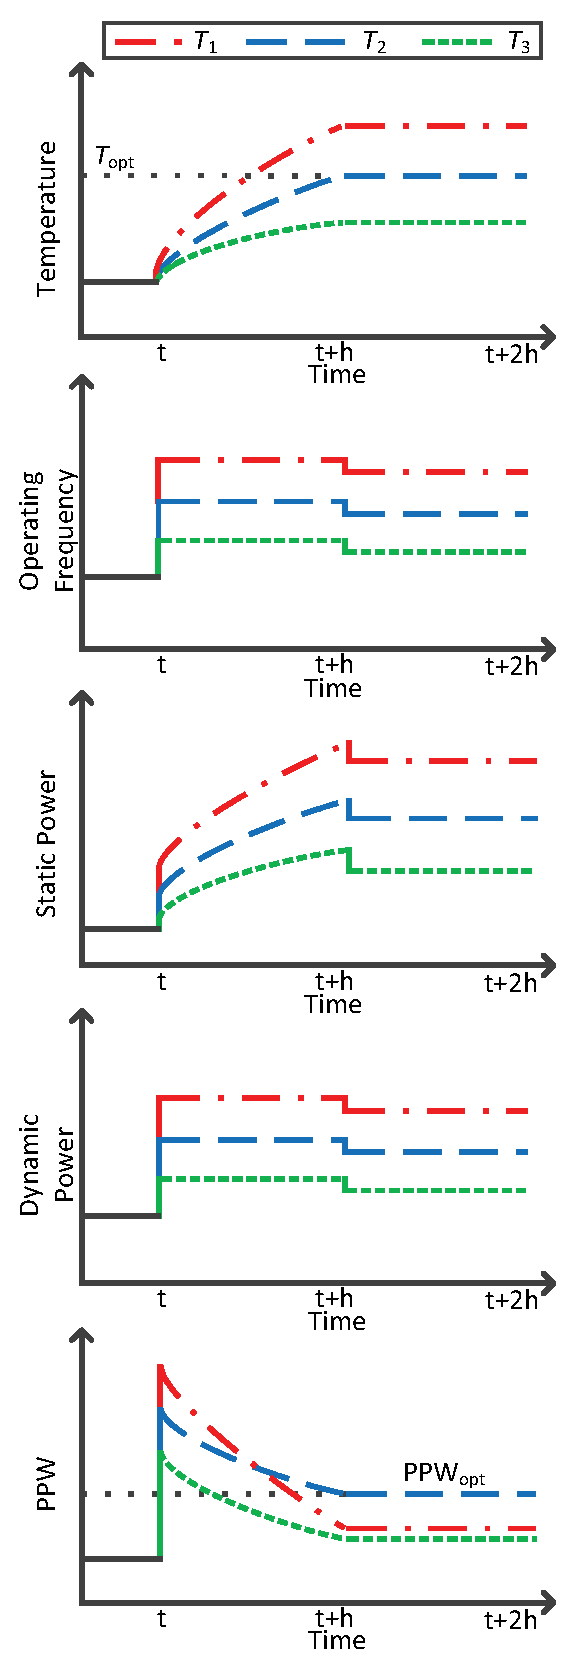
\includegraphics[width=\textwidth]{fig/ppw_boost_1.eps}\label{fig:ppw_boost_1}
\end{minipage}
}
\subfigure[Previous temperature is above $T_{opt}$.]{
\begin{minipage}{.3\linewidth}
\centering
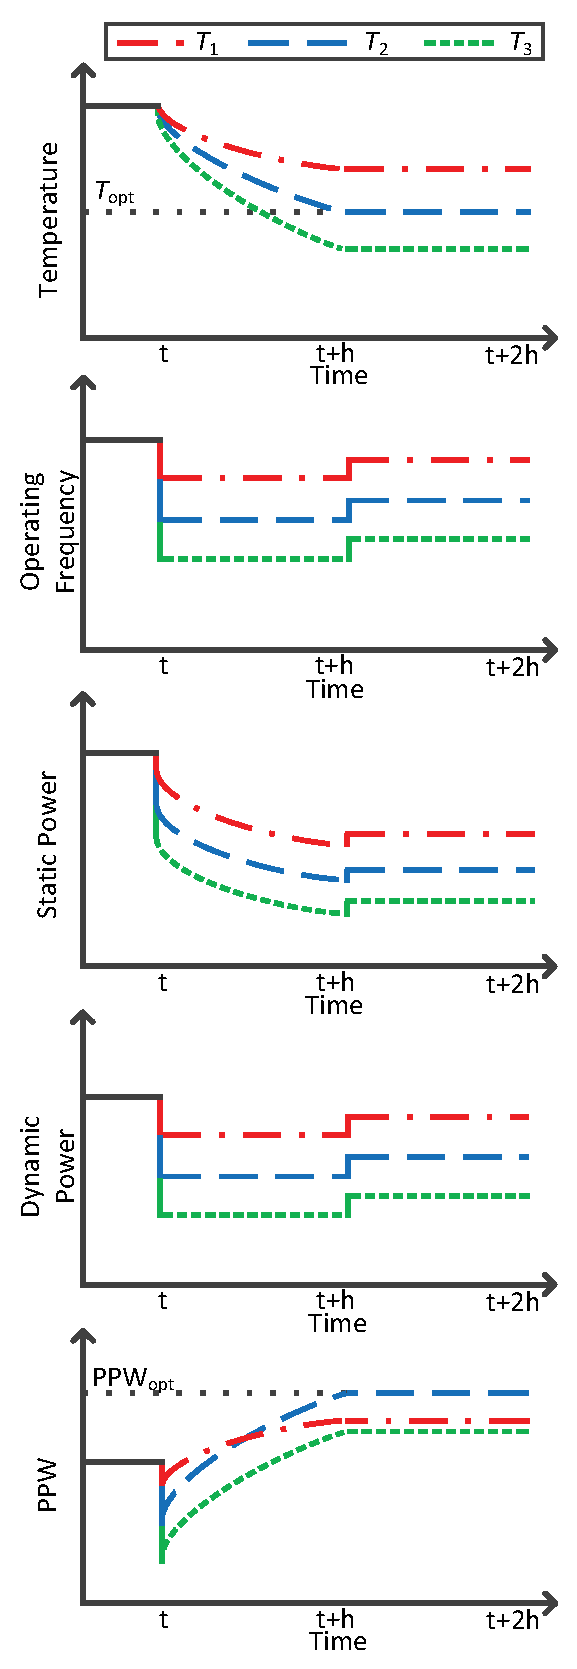
\includegraphics[width=\textwidth]{fig/ppw_boost_2.eps}\label{fig:ppw_boost_2}
\end{minipage}
}
\subfigure[Previous temperature is $T_{opt}$.]{
\begin{minipage}{.3\linewidth}
\centering
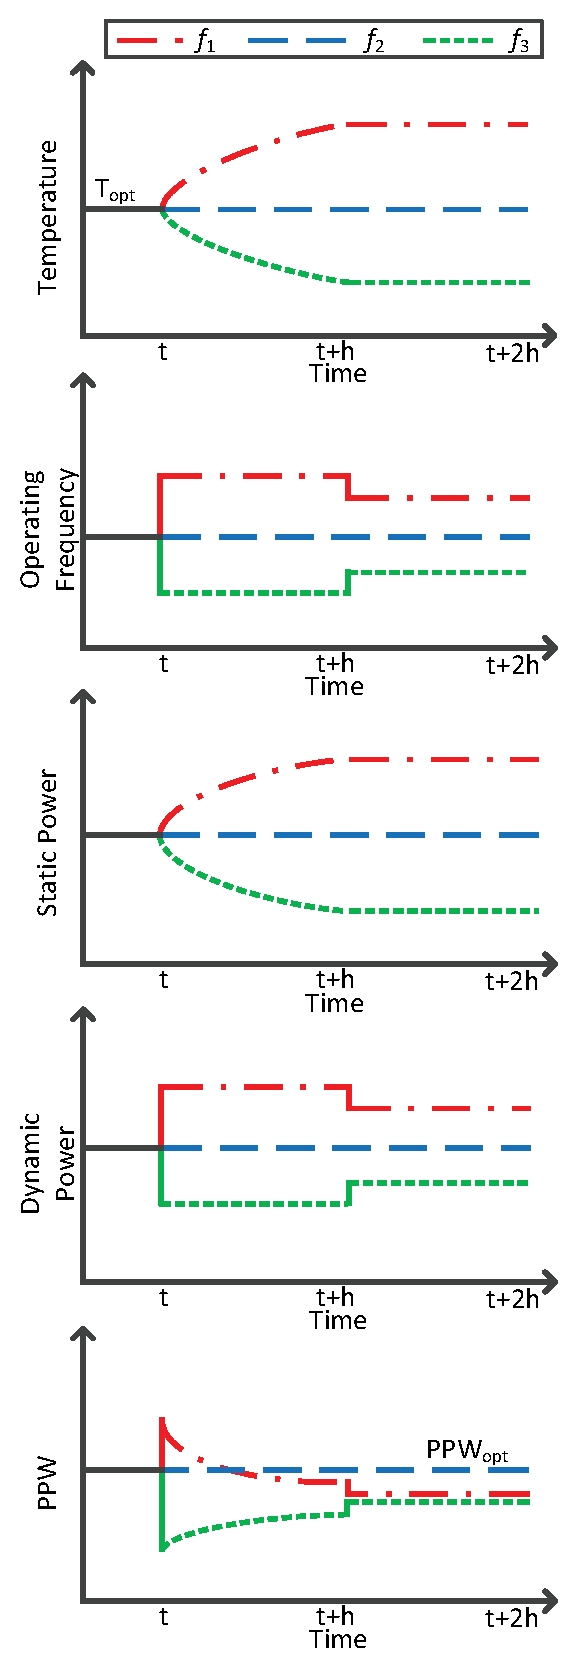
\includegraphics[width=\textwidth]{fig/ppw_boost_3.eps}\label{fig:ppw_boost_3}
\end{minipage}
}
\caption{Demonstration of changing temperature and the corresponding PPW. $f_{1}>f_{2}>f_{3}$, and $f_{2}$ can lead to $T_{opt}$ in $T(t+h)$.}
\label{fig:ppw_boost}
\end{figure*}

In order to find the position of the $(i+1)$-th core, we subtract the
temperature rise caused by power budget of $i$ active cores from $T_{opt}$,
and obtain $T_{rm}=T_{opt}-A_iP_i$. Next, in order to find which core can complement the impact of the fixed $i$ active cores best, we compare the performance of each of the rest $n-i$ cores when $T_{rm}$ is reached, and choose the core with maximum performance.

%One example of comparing two possible active core positions (the $j$-th core and $k$-th core are took as examples) is shown in Fig.x.
%By turning on $j$-th core only, the corresponding temperature rise of the chip is $a_{j}p_{j}$, where $p_{j}$ is the $j$-th elements in $P$ which should be determined by solving \eqref{eq:1_sim_opt_topt}. Assume $p_{j}$ is correctly computed, then the $T_{j}$ component (temperature rise at position $j$) of $a_{j}p_{j}$ should be the same as the $T_{opt}$, and $T_{k}$ component of $a_{j}p_{j}$ will be lower than $T_{opt}$. Instead, by turning on the $k$-th core only, the corresponding solved power value $p_{k}$ will heat the chip to $a_{k}p_{k}$, with its $T_{j}$ component being lower than $T_{opt}$ and its $T_{k}$ component just being equal to $T_{opt}$. Between the $j$-th core and $k$-th core, we prefer to turn on the $j$-th core, 


%because its cost $\left \| T_{opt}-a_{j}p_{j} \right \|_{2}$ (length of $a_{j}p_{j}-T_{th}$ in xx) in the optimization problem \eqref{eq:1_sim_opt_topt} is smaller than the cost $\left \| T_{opt}-a_{k}p_{k} \right \|_{2}$ of turning on the $k$-th core, as observed in Fig. x. The physical meaning is: by turning on the $j$-th core, the overall system temperature is closer to $T_{opt}$. With all cores' temperature lower than $T_{opt}$, the overall system temperature of turning on the $j$-the core is higher than that of turning on the $k$-th core.




\subsection{Energy-efficient power budgeting with optimal performance considering transient effects}
The power budgeting method introduced in Section $4.3$ is for steady state condition and serves mostly for illustration of the basic idea of the dynamic power budgeting method. It may work just fine on the aspect of reliability if the computed steady state power budget is followed strictly during the power management process. However, it is frequent that chip switches between high performance mode and high energy efficiency mode, it is also possible that power management makes false decisions occasionally, the computed steady state power budget is not suitable for such scenarios. Therefore, we develop a power budgeting method by considering previous transient thermal/power behaviors as follows.

Before we demonstrate any details, it's necessary to examine the PPW metric in transient state.
There are generally $3$ cases in transient state, the previous temperature is below $T_{opt}$, or above $T_{opt}$, or just $T_{opt}$. For each case, based on the target temperature, $3$ scenarios can be classified, target temperature above $T_{opt}$, or below $T_{opt}$ or just $T_{opt}$. We assume the operating frequency in one control cycle is fixed, therefore, the $3$ scenarios for each case can be viewed as with different operating frequencies, which are $f_{1}>f_{2}>f_{3}$, and by applying $f_{2}$, $T_{opt}$ can be reached in $T(t+h)$, where $h$ is the length of control cycle. We will talk each of the cases in details next.
%in order to improve the PPW of the core, it's necessary to improve the temperature, the difference is how much to improve. We assume the operating frequency in the process is fixed, the goal is to improve the PPW during $t$ and $t+h$, and maintain the temperature of $T_{t+h}$ until $t+2h$. $h$ is the length of control cycle.  Therefore, the $3$ senerios with different frequencies can also be classified by the target temperature by $T(t+h)$. For $f_{1}$, $T(t+h)$ will be higher than $T_{opt}$, $f_{2}$ will lead to $T_{opt}$ in $t+h$, and for $f_{3}$, $T_{t+h}$ will be lower than $T_{opt}$. 

We begin with the case where previous temperature is below $T_{opt}$, as Fig.~\ref{fig:ppw_boost_1} shows, for different frequencies, the temperature by the end of the $1^{st}$ control cycle will be different. And in the $2^{nd}$ control cycle, the temperature of all $3$ operating frequencies will remain constant, meaning they are in steady state from $t+h$ to $t+2h$.

Note that although $f_{1}>f_{2}>f_{3}$ is correct for both the control cycles, there is a sudden drop of frequency in $t+h$ for all cases, which comes from the fact that the power budget provided by our method to increase temperature to target temperature is higher than that of the target temperature in steady state. This means our method can provides "performance boost" when previous temperature is lower than target temperature.

Also as shown in Fig.~\ref{fig:ppw_boost_1}, PPW will temporarily increase dramatically in the beginning of the $1^{st}$ control cycle. The reason can be obtained from the definition of PPW as
\begin{equation}\label{eq:ppw_detail}
\text{PPW} = \frac{\left \| f \right \|_{1}}{\left \| P_{d}+P_{s}(T) \right \|_{1}},
\end{equation}
As shown in Fig.~\ref{fig:ppw_boost_1}, $f$ and $P_{d}$ will instantly change, however, $P_{s}$ is only relative to $T$, as the change of $T$ takes time, $P_{s}$ will be lower than its value in steady state for corresponding $f$ in the $1^{st}$ control cycle. Therefore, for the case where previous temperature is below $T_{opt}$, PPW will increase dramatically with the increase of $f$, especially for $f$ equals to or above $f_{2}$, PPW will temporarily exceed the optimal PPW of steady state, which means besides "performance boost", our method can also provides "PPW boost". Due to "performance boost", "PPW boost" is further increased. By the end of the $1^{st}$ control cycle, PPW for all cases will still be higher than that of corresponding temperature in steady state. For $f_{2}$, PPW in the $1^{st}$ control cycle remains higher than $\text{PPW}_{opt}$ in steady state.


%This means, when previous temperature is lower than $T_{opt}$, our method can provide a PPW higher than the $\text{PPW}_{opt}$ in steady state.
% For in the first case, $T(t+h)$ is higher than $T_{opt}$, PPW will gradually decrease, until $t+h$, it will be lower than optimal PPW. 

Then we focus on the case where previous temperature is above $T_{opt}$, as Fig.~\ref{fig:ppw_boost_2} shows, for all $3$ kinds of frequencies, contrary to the first case, to correct the previous over high temperature, we have to suffer from "performance deterioration" and "PPW deterioration". The "performance deterioration" comes from the fact that in order to reach target temperature by the end of the $1^{st}$ control cycle, the power budget given by our method is lower than that of corresponding target temperature in steady state. The reason of "PPW deterioration" is relatively the same as "PPW boost", in that contrary to $f$ and $P_{d}$, the change of $P_{s}$ takes time, therefore $P_{s}$ will be larger than that of steady state in the $1^{st}$ control cycle, resulting in a PPW less than the PPW in steady state. Note that the "performance deterioration" further deteriorate PPW, as by $T(t+h)$, PPW is still lower than that in steady state.
%as there is a boost in PPW at the beginning of $2^{nd}$ control cycle.


For the last case where previous temperature is $T_{opt}$, as Fig.~\ref{fig:ppw_boost_3} shows, for $f_{2}$, the power budget is the same as in steady state, therefore, we focus on the other $2$ scenarios. For $f_{1}$, because the target temperature is higher than $T_{opt}$, there is "PPW boost" in the $1^{st}$ control cycle. For $f_{3}$, it has to suffer from "PPW deterioration" due to lowering temperature.


We next focus on verifying the effectiveness of $T_{opt}$ in transient state, which equals to proving the overall PPW during a control cycle of $f_{2}$ is the highest among $f_{1}$, $f_{2}$ and $f_{3}$. We can see in Fig.~\ref{fig:ppw_boost}, no matter what previous temperature it is, the PPW of $f_{3}$ is always lower than that of $f_{2}$ in a control cycle. As for $f_{1}$, although the PPW of higher operating frequency will be higher than that of $f_{2}$ in the first half of the control cycle, the deviation of the target temperature from $T_{opt}$ makes the PPW of it lower than that of $f_{2}$ in the second half of the control cycle. Overall, the PPW of $f_{1}$ and $f_{2}$ is approximately the same. However, the PPW in the next control cycle is what sets them apart. By remaining the current temperature, the PPW of $f_{1}$ will be lower than that of $f_{2}$. Or, if the temperature is corrected to $T_{opt}$, the PPW will be even worse because of "PPW deterioration" mentioned above. Therefore, the PPW of applying $f_{2}$ in all circumstances will be maximum among $f_{1}$, $f_{2}$ and $f_{3}$.


% In the case where previous temperature is $T_{opt}$, As shown in Fig.~\ref{fig:ppw_boost}, 

% We can see in Fig.~\ref{fig:ppw_1_3}, compared to $f_{2}$, the PPW of $f_{1}$ is higher in the beginning of the control cycle, which is because $f_{1}$ is higher than $f_{2}$, and it takes time for $P_{s}$ to change. Because $T_{t+h}$ of $f_{1}$ is higher than $T_{opt}$, the PPW of $f_{1}$ will decrease faster than the PPW of $f_{2}$, which leads to lower PPW in the second half of the control cycle. For $f_{3}$, because $f_{3}$ is the lowest among all three cases, the PPW is also the lowest in the beginning. And $T(t+h)$ of $f_{3}$ is lower than $T_{opt}$, the PPW in the second half is still lower than the PPW of the second case. 




% by applying three different operating frequencies, $T(t+h)$ and PPW will change accordingly. 

% In the beginning, $f$ and $P_{d}$ change instantly, and the change of $T$ takes time, therefore, $P_{s}$ still remains high, which causes PPW to drop instantly at the beginning of $1^{st}$ control cycle. 



% In the meantime, because the decreasement of $f_{1}$ is less than $f_{2}$, the corresponding PPW drop of $f_{1}$ is also less. Yet the deviation from $T_{opt}$ in $t+h$ causes the PPW of $f_{1}$ in $t+h$ less than optimal PPW. For $f_{3}$, the largest drop in frequency causes the PPW to drop most dramaticly, and the lower temperature in $t+h$ than $T_{opt}$ leads to PPW lower than optimal in then end of the interval.  

% We can see for frequency lower than $f_{2}$, no matter the previous temperature is higher or lower than $T_{opt}$, the PPW in the interval will always be lower than the PPW of $f_{2}$. For frequency higher than $f_{2}$, no matter the previous temperature is higher or lower than $T_{opt}$, compared to the PPW of $f_{2}$, the PPW in the first half of the interval will be higher, and lower in the second half, and overall approximately the same. However, because the $T(t+h)$ is higher than $T_{opt}$, a further adjustment in the next control interval is required, which will will lead to major loss in PPW. Therefore, $T_{opt}$ is still effective in transient state.

With $T_{opt}$ being effective, the basic problem in dynamic power budgeting is to represent temperature rise $T_{c}(t+h)$ using the input power $P$ and initial temperature rise $T_{t}$. Once the formulation of $T_{c}(t+h)$ is available, we can input it into the basic optimization problem \eqref{eq:opt_topt}, and get the sub-optimal $P$ using the similar greedy based method presented in Section $4.3$.

For \eqref{eq:gt}, we can discrete this model using backward Euler's method, and get
\begin{equation}\label{eq:discrete_gt}
(\frac{C}{h}+G)\cdot T(t+h)=\frac{C}{h}T(t)+BP,
\end{equation}
and we are able to express $T_{c}(t+h)$ using $P$ and $T(t)$ as
\begin{equation}\label{eq:discrete_gt}
  \begin{split}
T_{c}(t+h)&=B^{T}T(t+h)\\
&=B^{T}(\frac{C}{h}+G)^{-1}T(h)+B^{T}(\frac{C}{h}+G)^{-1}BP.
  \end{split}
\end{equation}
%\emph{constant}

The cost function of the steady state power budgeting problem in
\eqref{eq:opt_topt} will be changed by using the new $T_c(t+h)$ for
transient case as
\begin{equation}\label{eq:cost_trans}
\|T_{opt} -  B^{T}(\frac{C}{h}+G)^{-1}T(h)+B^{T}(\frac{C}{h}+G)^{-1}BP\|_2.
\end{equation}
In order to simplify notation, we denote a new vector  
\begin{equation}
\bar{T}_{opt}=T_{opt} - B^{T}(\frac{C}{h}+G)^{-1}T(h),
\end{equation}
where $\bar{T}_{opt}$ has similar meaning of
$T_{opt}$ in steady state case, and it also accounts for the transient
thermal effects, i.e., current temperature's impact on power
budget. Also, we denote a new matrix 
\begin{equation}
\bar{A} = B^{T}(\frac{C}{h}+G)^{-1}B, 
\end{equation}
which works similarly as matrix $A$ in steady
state case, but accounts for transient thermal effect. The power
budgeting optimization problem for transient case is updated as 
\begin{equation}\label{eq:temp_ts_opt}
\begin{split}
\text{minimize } &  \left \| \bar{T}_{opt}-\bar{A}P \right \|_{2}\\
\text{subject to} &\left\{
\begin{array}{lr}
\text{card}(P) = n_{a},\\
\bar{A}P \preceq \bar{T}_{th}.\\
\end{array}
\right.
\end{split}
\end{equation}
Now dynamic power budgeting can be
applied by following the steps in steady state power budgeting presented in
Section $4.3$, just with \eqref{eq:sim_opt_topt} replaced
by \eqref{eq:temp_ts_opt}.


